\section{Approach}
\label{sec:approach}

The goal of this paper is to develop a method for automatically generating pattern coloring suggestions. The system should take as input a target pattern template, along with any additional user-provided constraints, and output a wide variety of colorings that evoke the coloring style desired by the user.

A \emph{pattern template} specifies which regions in an image can be colored in, and which regions must map to the same color. For example, an image of a flower on a background may have a template that specifies all petals of the flower must be the same color, and all background regions must be the same color. In the rest of the paper, we refer to a set of regions that map to the same color as a \emph{color group}. Figure~\ref{fig:teaser} shows an example of a pattern template visualized in grayscale, where each different lightness level identifies a different color group. This pattern template representation is relatively easy to author from images composed of segments, such as web designs, renderings of 3D scenes, and line drawings. In this paper, we focus primarily on 2D graphic design patterns. 

To generate attractive pattern colorings, a reasonable first step is to enforce that the colors used are `compatible' with one another, for some definition of color compatibility. Figure~\ref{fig:ColorCompatOnly} shows several patterns whose colors receive a high score under the color compatibility model of O'Donovan et al.~\shortcite{ODonovan}.~\remark{Make this figure.} While high-scoring colorings do exhibit a great degree of diversity, most of them simply don't look very good. They exhibit several problems, such foreground regions that blend into the background, and background regions that are too `loud' in color. Furthermore, color compatibility is a universal notion: it is not clear how to adapt it to match the style of a particular artist or the preferences of a particular user.

\begin{figure}
\centering
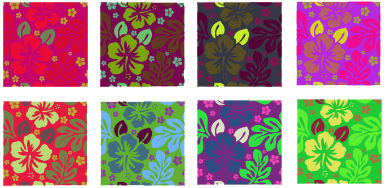
\includegraphics[width=\columnwidth]{figs/colorCompatOnly}
\caption{Patterns whose colors receive high scores under the color compatibility model of O'Donovan et al.~\shortcite{ODonovan}. Many patterns exhibit problems such as adjacent equi-luminant regions and excessively saturated backgrounds.~\remark{Figure not final.}}
\label{fig:ColorCompatOnly}
\end{figure}

While compatibile colors are an important component of attractive pattern colorings, they do not tell the whole story. The notion of color compatibility, whether implemented via the O'Donovan model or any other, considers colors abstractly: it does not take into account how they will be spatially used in the pattern. Large, background regions are colored differently than smaller, scattered `accent' regions; a thin, ribbon-like region against an empty field is colored differently than a thin region amidst a mass of similar regions.

Rather than develop a specialized algorithm for this problem, we exploit the insight that both of these concerns---color harmony and spatial consistency---can be encoded in the extremely general framework of probabilistic factor graphs~\cite{FactorGraphs}. In the next section, we develop a data-driven factor graph model that can be trained on example colored patterns and sampled to generate new coloring suggestions. The factor graph formalism allows us to leverage existing models of color compatibility, to plug in additional coloring constraints in response to available user input, and to capture the characteristics of desired styles through established machine learning techniques.

To build a data-driven model, we require a source of training data. For the experiments in this paper, we used a dataset of colored patterns scraped from the Colourlovers website. The dataset contains 100 colored patterns for each of 82 artists---8200 patterns in total. The artists were chosen based on TODO.~\remark{Chosen based on popularity? Also, describe the image preprocessing we do (because we dont' have access to the original vector artwork?)}